\documentclass[a4paper, 12pt]{article}

\usepackage[sort&compress]{natbib}
\bibpunct{(}{)}{;}{a}{}{,} 

\usepackage{amsthm, amsmath, amssymb, mathrsfs, multirow, url}
\usepackage{caption}
\usepackage{subcaption}
\usepackage{makecell,booktabs,siunitx}
\usepackage{graphicx} 
\usepackage{ifthen} 
\usepackage{amsfonts}
\usepackage[usenames]{color}
\usepackage{placeins}
%\usepackage{fullpage}

\usepackage[margin=1in]{geometry}
\usepackage{fancyhdr}
\pagestyle{fancy}
\lhead{\scalebox{0.25}{

\includegraphics{resone-logo.png}}
%\includegraphics{R-dot-one.png}}
\rhead{
{\small 
\url{https://www.researchers.one/article/2019-03-4}} % fill in URL here
}
}

\usepackage{xspace}
%\usepackage{amsmath}
%\usepackage{natbib}
%\usepackage{comment}
%\usepackage{graphicx}
%\usepackage{authblk}
\usepackage[colorlinks=true,citecolor=blue]{hyperref}

\newcommand{\bi}{\begin{itemize}}
\newcommand{\ei}{\end{itemize}}


\newcommand{\ave}[1]{\left\langle#1 \right\rangle}
\newcommand{\gamble}[1]{{\sc#1}}
\newcommand{\person}[1]{{\sc#1}}
\newcommand{\concept}[1]{{\sc#1}}
\newcommand{\elabel}[1]{\label{eq:#1}}
\newcommand{\eref}[1]{(Eq.~\ref{eq:#1})}
\newcommand{\ceref}[2]{(\ref{eq:#1}#2)}
\newcommand{\Eref}[1]{Equation~(\ref{eq:#1})}
\newcommand{\flabel}[1]{\label{fig:#1}}
\newcommand{\fref}[1]{Fig.~\ref{fig:#1}}
\newcommand{\Fref}[1]{Figure~\ref{fig:#1}}
\newcommand{\tlabel}[1]{\label{tab:#1}}
\newcommand{\tref}[1]{Tab.~\ref{tab:#1}}
\newcommand{\Tref}[1]{Table~\ref{tab:#1}}
\newcommand{\seclabel}[1]{\label{sec:#1}}
\newcommand{\secref}[1]{Sec.~\ref{sec:#1}}
\newcommand{\Secref}[1]{Section~\ref{sec:#1}}
\newcommand{\nmax}{{n_{\text{max}}}\xspace}
\newcommand{\gens}{g_\text{e}}
\newcommand{\gtime}{\bar{g}}
\newcommand{\gi}{g^{(i)}}
\newcommand{\Ito}{It\^{o}\xspace}
\newcommand{\etal}{{\it et~al.}\xspace}
\newcommand{\apriori}{{\it a priori}\xspace}
\newcommand{\ie}{{\it i.e.}\ }
\newcommand{\etc}{{\it etc.}\xspace}
\newcommand{\eg}{{\it e.g.}\ }
\newcommand{\cf}{{\it c.f.}\ }
\newcommand{\vv}{{\it v.v.}\ }
\newcommand{\err}{\epsilon}
\newcommand{\gensst}{g_{\text{est}}}
\newcommand{\be}{\begin{equation}}
\newcommand{\ee}{\end{equation}}
\newcommand{\bea}{\begin{eqnarray}}
\newcommand{\eea}{\end{eqnarray}}
\newcommand{\D}{\Delta}
\newcommand{\yn}[1]{{y^{(#1)}}}
\newcommand{\xin}[1]{{\xi^{(#1)}}}
\newcommand{\Wn}[1]{{W^{(#1)}}}
\newcommand{\mun}[1]{{\mu^{(#1)}}}
\newcommand{\sigman}[1]{{\sigma^{(#1)}}}
\newcommand{\sigmac}{{\sigma_\rho}}

\newcommand{\ND}{\mathcal{N}} % Normal Distribution
\newcommand{\sigmat}{\tilde{\sigma}}
%\newcommand{\var}[1]{\text{var}(#1)}
\newcommand{\MK}[1]{{\it ***MK: #1 MK***}}
\newcommand{\OP}[1]{{\it ***OP: #1 OP***}}
\newcommand{\YB}[1]{{\it ***YB: #1 YB***}}
\renewcommand{\AA}[1]{{\it ***AA: #1 AA***}}

\title{Why are we weighting? \\
{\small A mechanistic model for probability weighting}}
\author{
Ole Peters\footnote{London Mathematical Laboratory, 8 Margravine Gardens, London W6 8RH, UK and Santa Fe Institute, 1399 Hyde Park Road, Santa Fe, 87501 NM, USA. Email: \texttt{o.peters@lml.org.uk}} \;
Alexander Adamou\footnote{London Mathematical Laboratory, 8 Margravine Gardens, London W6 8RH, UK. Email: \texttt{a.adamou@lml.org.uk}} \;
Mark Kirstein\footnote{London Mathematical Laboratory, 8 Margravine Gardens, London W6 8RH, UK. Email: \texttt{m.kirstein@lml.org.uk}} \;
Yonatan Berman\footnote{London Mathematical Laboratory, 8 Margravine Gardens, London W6 8RH, UK. Email: \texttt{y.berman@lml.org.uk}} 
}
\date{\today}

\begin{document}
\begin{titlepage}
	\maketitle
\thispagestyle{fancy}

\begin{abstract}
\noindent 
Behavioural economics provides labels for patterns in human economic behaviour. 
Probability weighting is one such label. It expresses a mismatch between probabilities used in a formal model of a decision problem (\ie model parameters) and probabilities inferred from real people's behaviour faced with the modelled decision problem (the same parameters estimated empirically). The inferred probabilities are called ``decision weights.'' 
It is considered a robust observation that decision weights are higher than probabilities for extreme events, and (necessarily, because of normalisation) lower than probabilities for common events. 
We formalise this observation as an observer and a decision maker using different probability distributions to model the outcome of an experiment.
We show how the specific disagreement arises from the decision maker having to estimate probabilities as frequencies in a time series, whereas the observer may know them a priori. 
\vspace{1em}

\noindent\textsf{\textbf{Keywords}} ~ Decision Theory, Prospect Theory, Probability Weighting, Ergodicity Economics
\vspace{.5em}

\noindent\textsf{\textbf{JEL Codes}} ~
% \href{https://www.aeaweb.org/econlit/jelCodes.php?view=jel#B}{%
% B16, % HET: Quantitative and Mathematical 
\href{https://www.aeaweb.org/econlit/jelCodes.php?view=jel#C}{%
% C60		% Mathematical Models
% $\cdot$
C61		% Optimization Techniques • Programming Models • Dynamic Analysis
$\cdot$
}%
\href{https://www.aeaweb.org/econlit/jelCodes.php?view=jel#D}{%
D01 	% Microeconomic Behaviour: Underlying Principles
$\cdot$
D81 	% Criteria for Decision-Making under Risk and Uncertainty
% $\cdot$
% D9		% Micro-Based behavioural Economics 
}
\end{abstract}
\end{titlepage}
 
\setcounter{page}{2}		% titlepage=page 1, continue with page 2

%\section{Introduction and key observation}
%In this paper, we provide a mechanistic explanation of the phenomenon traditionally labelled as probability weighting, which originates in prospect theory.\footnote{\cite{TverskyKahneman1992} For a useful survey see \cite{Barberis2013}.} We find it to be a beneficial behavioural pattern instead of a systematic irrational bias. 
 
%We find that the phenomenon is a reasonable way to cope with uncertainty in the real world of a specific kind.
 
%Some processes in nature have random outcomes. Model of such processes may therefore comprise random variables and stochastic processes. However, on top of the inherent stochasticity of nature captured in such a model, there is additional model uncertainty, often referred to as radical or fundamental uncertainty. In its mildest form, model uncertainty can manifest itself in parametric uncertainty within a class of models (\eg uncertainty in the estimates of the mean of a normal distribution). More severe forms are conceivable (\eg uncertainty about the correct class of models/probability distributions) but are not necessary for our mechanistic explanation of probability weighting.
% 
%We thereby conceptualise probability weighting as a reasonable pattern in human behaviour to cope with the fundamental uncertainty in the real world.
%\OP{We don't invoke radical uncertainty. Just regular uncertainty in parameter estimates is sufficient.}

%\paragraph{Organisation of the paper} The remainder is organised as follows \ldots
%We begin by discussing the necessity for using decision weights that are greater than the probabilities for rare events. Next, we discuss as an example how the same effect can arise when repeatedly facing prospects with a Gaussian random variable whose mean fluctuates in time.
%
%Finally, we calculate analytically, and plot, the probability weighting curves one would expect on this basis. We compare these to the empirical results summarised by \cite{Barberis2013}, and we comment on the function fitted to these data by \cite{TverskyKahneman1992}.
%
%Our work contributes to the growing field of ergodicity economics
%\cite{Peters2019b} where decision makers are modelled as behaving optimally over time (as opposed to optimally in a statistical-ensemble sense).


\section{Introduction}
{\it Probability weighting} is a concept that originated in prospect theory. It is one way to conceptualise a pattern in human behaviour, of caution with respect to formal models.
This is best explained by a thought experiment, in which  
\bi
	\item a \textit{disinterested observer} (DO), such as an experimenter, tells
	\item a \textit{decision maker} (DM)
\ei
that an event occurs with some probability. The DO observes DM's behaviour (\eg gambling on the event), and finds it consistent with a behavioural model (\eg expected-utility optimization) in which the DM uses a probability that differs systematically from what the DO has declared. The apparent probabilities, inferred from the DM's decisions, are called ``{\it decision weights}.'' We will adopt this nomenclature here: 
% 
\bi
	\item By ``\textit{probabilities,}'' expressed as probability density functions (PDFs) and denoted $p(x)$, we will mean the numbers specified by a DO.
	\item By ``\textit{decision weights,}'' also expressed as PDFs and denoted $w(x)$, we will mean the numbers that best describe the behaviour of a DM in the DO's behavioural model.\footnote{In the literature, decision weights are not always normalised, but for simplicity we will work with normalised decision weights. Mathematically speaking, they are therefore proper probabilities even though we don't call them that. Our results are unaffected because normalising just means dividing by a constant (the sum or integral of the non-normalised decision weights).}
\ei
Here, $x$ is a realisation of a random variable, $X$. For example, $X$ might be the payout of a gamble which the DM is invited to accept or decline.

Specifically, it is consistently observed that decision weights, $w(x)>p(x)$ (used by DMs), are higher than probabilities,  $p$ (declared by DOs), for extreme events (with small $p$). 
This observation is often summarised visually by comparing 
\bi
\item cumulative density functions (CDFs) for probabilities, denoted 
\be
F_p(x)=\int_{-\infty}^x p(s) ds
\ee
\item and CDFs for decision weights, denoted
\be
F_w(x)=\int_{-\infty}^x w(s) ds ~.
\ee
\ei
In \fref{TK1992} we reproduce the first such visual summary from \citet[p.~310]{TverskyKahneman1992}.

\begin{figure}[!htb]
\centering
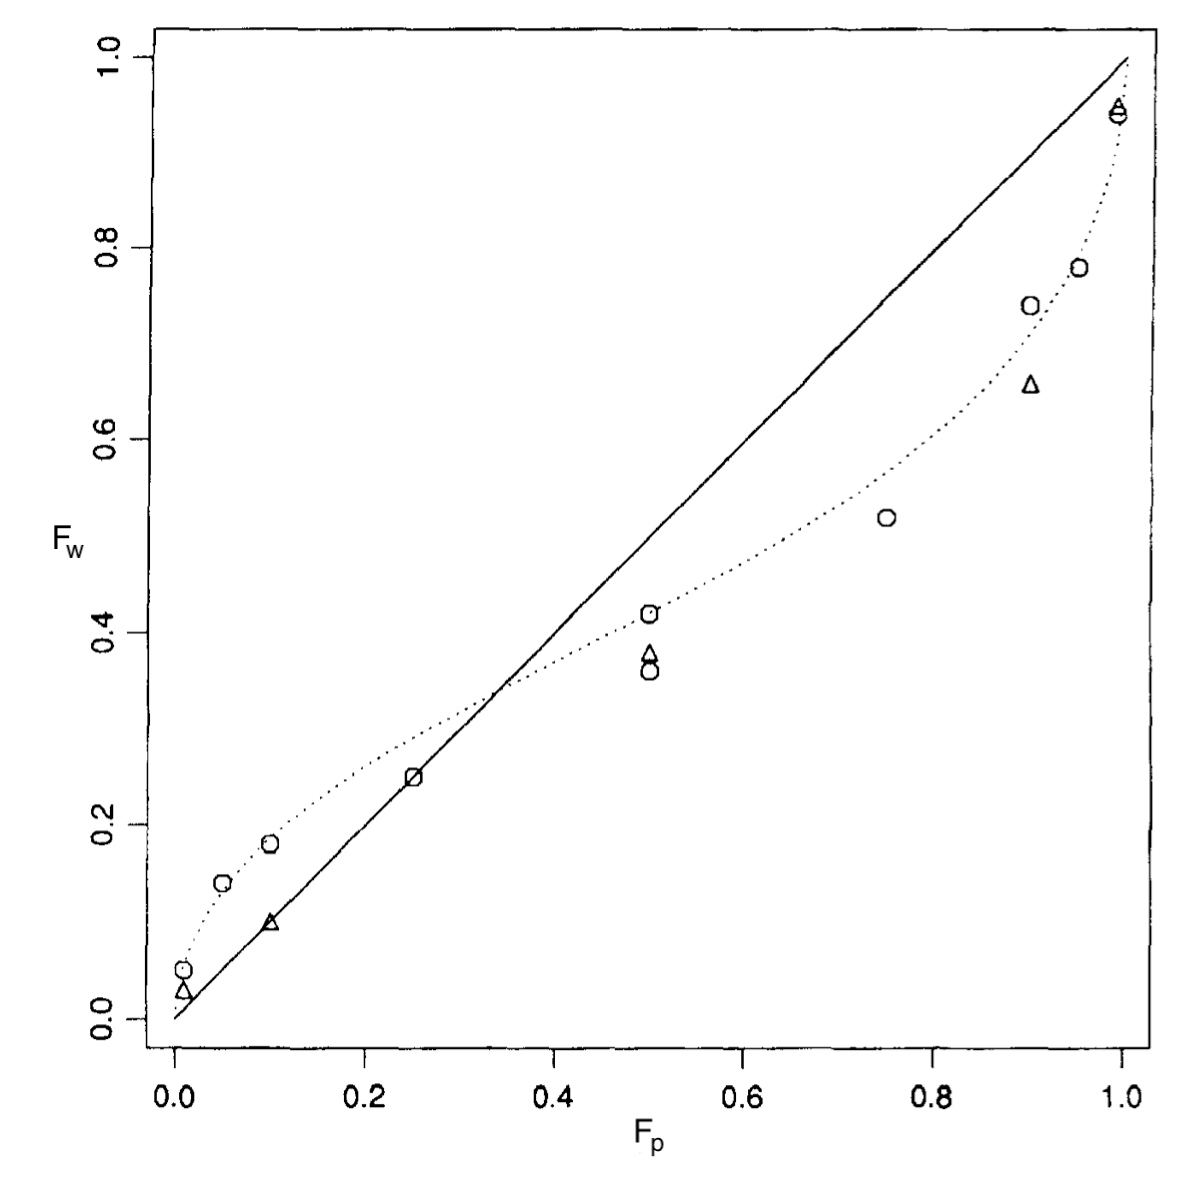
\includegraphics[width=0.5\textwidth]{./figs/TK1992.PNG}
\caption{{\bf Empirical phenomenon of probability weighting.} Cumulative decision weights $F_w$ (used by decision makers) versus cumulative probabilities $F_p$ (used by disinterested observers), as reported by \citet[p.~310, Fig. 1, relabelled axes]{TverskyKahneman1992}. The figure is to be read as follows: pick a point along the horizontal axis (the cumulative probability $F_p$ used by a DO) and look up the corresponding value on the vertical axis of the dotted inverse-S curve (the cumulative decision weight $F_w$ used by a DM). Low cumulative probabilities (left) are exceeded by their corresponding cumulative decision weights, and for high cumulative probabilities it's the other way around. It's the inverse-S shape of the curve that indicates this qualitative relationship.}
\flabel{TK1992}
\end{figure}

As a final piece of nomenclature, we will use the terms \textit{location}, \textit{scale}, and {\it shape} when discussing probability distributions. Consider a standard normal distribution $\ND(0,1)$ -- here, the parameters indicate location 0 and squared scale 1 (for a Gaussian the location is the mean and scale is the standard deviation). For a general random variable $X$, with arbitrary parameters for location $\mu_X$ and scale $\sigma_X$, the transformation in \eref{SN} obtains the identically-shaped location-0 and scale-1 distribution for the so standardised random variable
\be \elabel{SN}
	Z = \frac{X-\overbrace{\mu_X \mathstrut}^{\text{location}}}{\underbrace{\sigma_X\mathstrut}_{\text{scale}}}
%		~, \qquad \qquad Z \sim \ND(0,1
~.
\ee
Thus the PDF of $Z$, $p(z)$, is a density with location $\mu_Z=0$ and scale $\sigma_Z=1$. In a graph of a distribution, a change of location shifts the curve to the left or right, and a change in scale shrinks or blows up the width of its features. Neither operation changes the {\it shape} of the distribution: two distributions have the same {\it shape} if they can be made to coincide through the linear transformation in \eref{SN}.

% We will show below that these observations are predicted by considerations of uncertainty about probabilities, or more generally by uncertainty about model parameters.


\section{Probability weighting as a difference between models} \seclabel{ModelDiff}

Behavioural economics interprets \fref{TK1992} as evidence for a cognitive bias of the DM, an error of judgement. We will keep a neutral stance. We don't assume the DO to know ``the truth'' -- he has a model of the world. Nor do we assume the DM to know ``the truth'' -- he has another model of the world. From our perspective \fref{TK1992} merely shows that the two models differ. It says nothing about who is right or wrong. This is true even in the context of a lab experiment, as we discuss in detail in \secref{Reasons_for}.

\subsection{The inverse-S curve\seclabel{The_inverse}}
\subsubsection{Tversky and Kahneman}
\citet{TverskyKahneman1992} chose to fit the empirical data in \fref{TK1992} with the following function
%\footnote{\Eref{correspondence} is the consensus functional form in the community \cite{Barberis2013}. \OP{Maybe not quite, given that we fit another function later. We could introduce Latimore's function hiere.}}
% 
\be
\elabel{correspondence}
\tilde{F}^{TK}_w\left(F_p; \gamma\right) = \left(F_p\right)^\gamma \frac{1}{\left[\left(F_p\right)^\gamma+\left(1-F_p\right)^\gamma\right]^{1/\gamma}} ~.
\ee
We note that no mechanistic motivation was given for fitting this specific family of CDFs (parameterised by $\gamma$). The motivation is purely phenomenological: with $\gamma<1$, this family ``looks a bit like the data.''
% 
The function $\tilde{F}^{TK}_w\left(F_p; \gamma \right)$ has only one free parameter, $\gamma$. For $\gamma=1$ it is the identity, and the CDFs coincide, $\tilde{F}^{TK}_w\left(F_p\right)=F_p$. Further, $\tilde{F}^{TK}_w$ has the following property: any curvature moves the intersection with the diagonal away from the mid-point $1/2$. This means if the function is used to fit an inverse-S (where $\gamma<1$), the fitting procedure itself introduces a shift of the intersection to the left. Because of this, we consider the key observation to be the inverse-S shape, whereas the shift to the left may be an artefact of the function chosen for the fit. 
%We will see below that the curvature and shift correspond to different parts of a mechanistic explanation of the phenomenon.

\subsubsection{Scale, location, and the inverse-S}
We now make explicit how the robust qualitative observation of the inverse-S shape in \fref{TK1992} emerges when the DM uses a larger scale in his model of the world than the DO. 
%This can have numerous reasons, to which we will return in \secref{Reasons_for}. 
%For now, suffice it to say that precaution is an obvious one: any uncertainty the DM wishes to include in his model in addition to what the DO includes will translate into a greater scale for the DM's distribution and therefore into an inverse-S shape for any unimodal (peaked) distribution when cumulative densities are compared.

We illustrate this with a Gaussian distribution.
Let's assume that a DO models an observable $x$ -- which will often be a future change in wealth -- as a Gaussian with location $\mu$ and variance $\sigma^2$. And let's further assume that a DM 
%(for whatever reason, perhaps caution) 
models the same observable as a Gaussian with the same location, $\mu$, but with a greater scale, so that the variance is $(\alpha\sigma)^2$. The DM simply assumes a broader range -- $\alpha$ times greater -- of plausible values, left panel of \fref{probability_dists}.

\begin{figure}[htb]
\centering
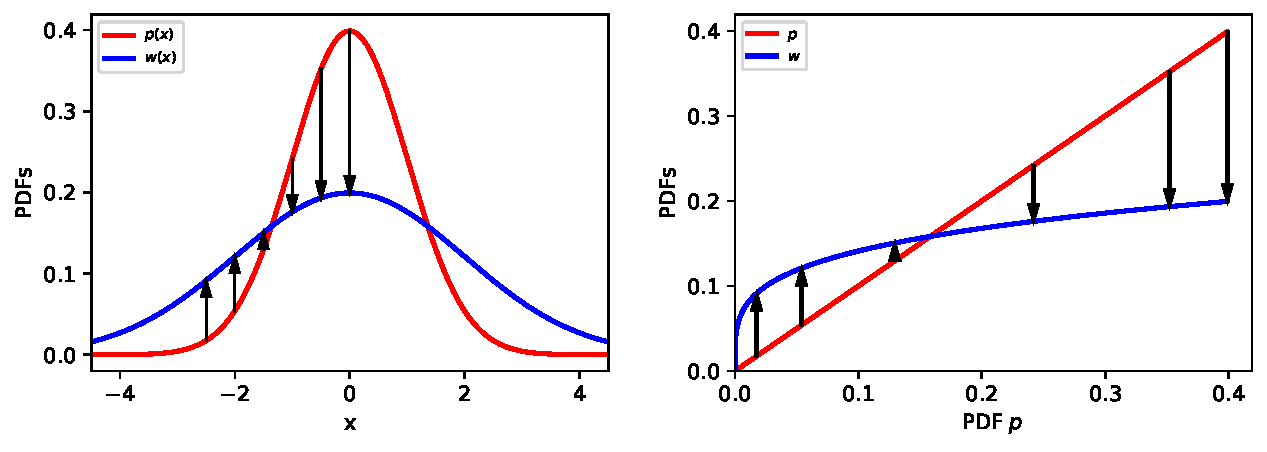
\includegraphics[width=\textwidth]{./figs/density_map.pdf}
\caption{{\bf Mapping PDFs.} Left: probability PDF (red), estimated by a DO; and decision-weight PDF (blue), estimated by a DM. The DO models $x$ with a best estimate for the scale (standard deviation) and assumes the true frequency distribution is the red line. The DM models $x$ with a greater scale (here 2 times greater, $\alpha=2$), and assumes the true frequency distribution is the blue line. Comparing the two curves, the DM appears to the DO as someone who over-estimates probabilities of low-probability events and underestimates probabilities of high-probability events, indicated by vertical arrows.
Right: the difference between decision weights and probabilities can also be expressed by directly plotting, for any value of $x$, the decision weight {\it vs.} the probability observed at $x$. This corresponds to a non-linear distortion of the horizontal axis. The arrows on the left correspond to the same $x$-values as on the right. They therefore start and end at identical vertical positions as on the left. Because of the non-linear distortion of the horizontal axis, they are shifted to different locations horizontally.}
\flabel{probability_dists}
\end{figure}
%\subsection{Repetition and location uncertainty}
%
%Let's stay with the investment example, and again say annual logarithmic returns are Gaussian-distributed. Let's also assume (somewhat unrealistically) that we know the variance of these returns to be $\sigma_1^2$, with certainty.
%
%Finally, we assume that the mean of the returns fluctuates. Over time, we don't always draw from the same Gaussian, but sometimes from one with a higher mean and sometimes from one with a lower mean.
%We implement this as follows: first, generate a mean, $\gamma$, from a Gaussian distribution $\gamma \sim \ND(\mu, \sigma_2^2)$. Then draw a return from a Gaussian with this mean and variance $\sigma_1^2$, meaning $g\sim\ND(\gamma,\sigma_1^2)$. Over time, the total log return is just the sum of the annual log returns, and it is equivalent to the total log return that would be generated with a Gaussian with known mean and higher variance, $g\sim \ND(\mu,\sigma_1^2+\sigma_2^2)$.
%
%Considering a single round, a DO might well use the best estimate for $\gamma$, which is $\mu$, and the known variance $\sigma_1^2$, so that $g_p\sim \ND(\mu,\sigma_1^2)$. A DM, on the other hand, who has to live with the consequences of what happens in a long sequence realizations of $g$ would use $g_w\sim \ND(\mu,\sigma_1^2+\sigma_2^2)$. Again, the situations and incentives of the DO and the DM are different, leading them to use different models (the same models as in \Secref{Survival})
%
%\section{Analysis of the Gaussian case}
%The point of the previous two sub-sections was to illustrate two different ways in which uncertainty or fluctuations in parameters lead to behaviour by a DM that leads to greater decision weights for extreme events than the probabilities a DO might assign to them. In the first case, the DO uses the best estimate, rather than a conservative estimate of the variance. In the second case, the DO assumes no fluctuations in the mean return.
%
%Both DO models give $g_p\sim\ND(\mu,\sigma_1^2)$, whereas the DM will choose the model $g_w \sim \ND(\mu,\sigma_1^2+\sigma_2^2)$.

Generically, if the DM uses a greater scale in his model, then decision weights are higher than probabilities for low-probability events, and (because of normalisation), lower than probabilities for high-probability events. We can express this by plotting, for any value of $x$, the decision weight {\it vs.} the probability observed at $x$, right panel of \fref{probability_dists}.

%\begin{figure}[htb]
%\centering
%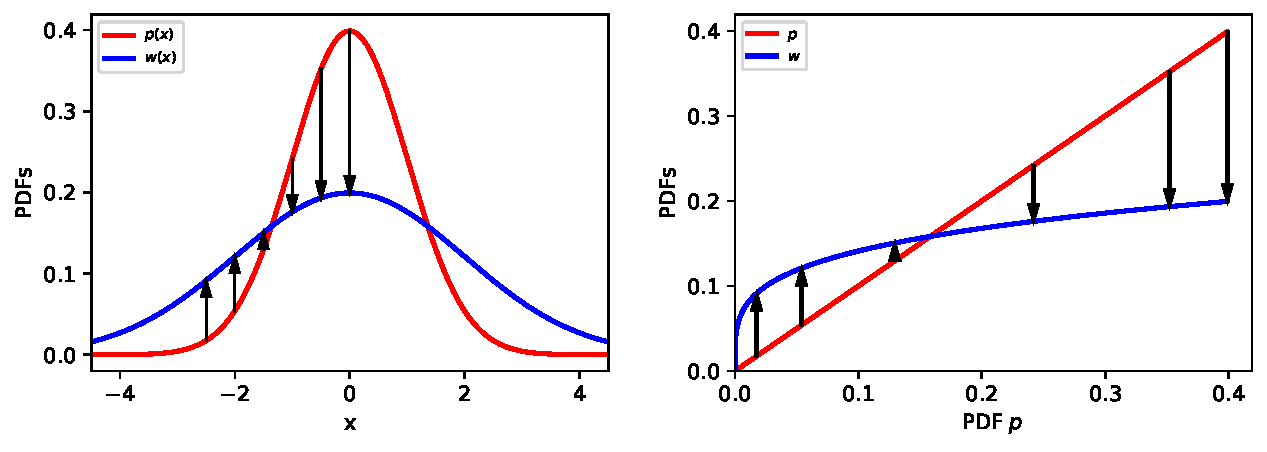
\includegraphics[width=0.7\textwidth]{./figs/density_map.pdf}
%\caption{Decision weight density (used by a DM) vs. probability density (used by a DO) for the Gaussian model (blue), compared to the diagonal (black dashed) where DM and DO use the same parameters. For low probabilities, the decision weights are higher than the probabilities; for high probabilities they are lower.}
%\flabel{probability_weights}
%\end{figure}

In the Gaussian case we can write the distributions explicitly
\be \elabel{DecisionW}
	w(x)=\frac{1}{\sqrt{2\pi (\alpha \sigma)^2}}\exp\left[\frac{-(x -\mu )^2}{2 (\alpha \sigma)^2}\right]
\ee
and
\be
	p(x)=\frac{1}{\sqrt{2\pi \sigma^2}}\exp\left[\frac{-(x -\mu )^2}{2 \sigma^2}\right] ~,
\elabel{p}
\ee
% 
and solve \eref{p} for $(x -\mu)^2$, substitute that in \eref{DecisionW}, and obtain the following expression for decision weights directly as a function of probabilities
\be
w(p)= p^{\frac{1}{\alpha^2}} \frac{\left(2\pi\sigma_1^2\right)^{\frac{1-\alpha^2}{2\alpha^2}}}{\alpha} ~,
\elabel{w_of_p}
\ee
which is precisely what's plotted in the right panel of \fref{probability_dists}. As a sanity check, consider the shape of the $w(p)$ (blue curve, right panel \fref{probability_dists}): for a given value of $\alpha$, it is just a power law in $p$ with some pre-factor that ensures normalization. If $\alpha>1$ it means that the DM uses a greater standard deviation than the DO. In this case, the exponent of $p$ satisfies $\frac{1}{\alpha^2}<1$, and the blue curve is above the diagonal for small arguments and below it for large arguments.

Alternatively, we can express the difference between models by plotting the CDFs $F_w$ and $F_p$. We do this in \fref{TwoCDFs}, where the inverted S emerges purely from the DM's greater assumed scale, $\alpha \sigma$.

\begin{figure}[!htb]
\centering
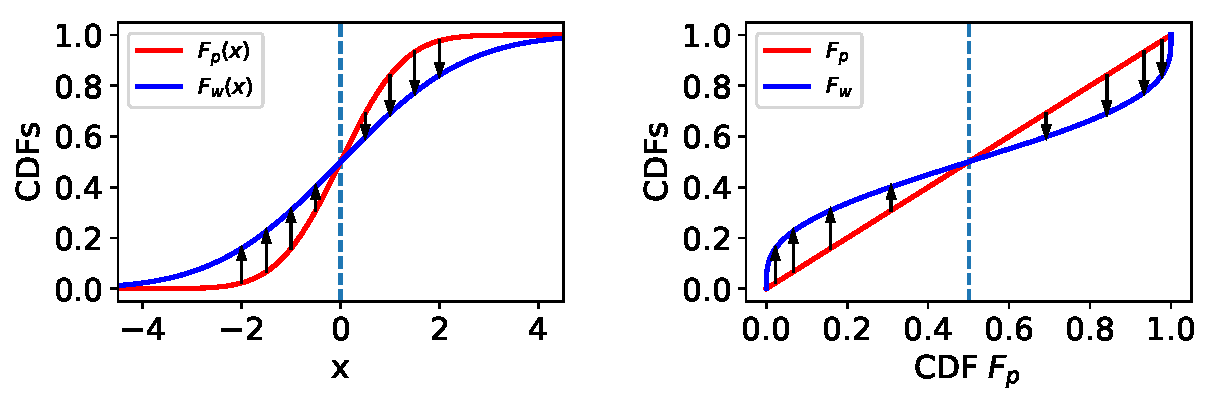
\includegraphics[width=\textwidth]{./figs/GaussianFvsXtoWvsP.pdf}
\caption{{\bf Mapping CDFs.} 
Left: The DO assumes the observable $X$ follows Gaussian distribution $X \sim \ND(0,1)$, which results in the red CDF of the standard normal, $F_p(x) = \Phi_{0,1}(x)$. The DM is more cautious, in his model the same observable $X$ follows a wider Gaussian distribution, $X \sim \ND(0,3)$ depicted by $F_w(x)$ (blue). 
% 
Following the vertical arrows (left to right), we see that for low values of the event probability $x$ the DM's CDF is larger than the DO's CDF, $F_p(x) < F_w(x)$; the curves coincide at 0.5 because no difference in location is assumed; necessarily for large values of the event probability $x$ the DM's CDF must be lower than the DO's.
Right: the same CDFs as on the left but now plotted not against $x$ but against the CDF $F_p$. Trivially, the CDF $F_p$ plotted against itself is the diagonal; the CDF $F_w$ now displays the generic inverse-S shape known from prospect theory. The arrows start and end at the same vertical values as on the left. Because the horizontal axis is has been non-linearly stretched (as the argument changed from $x$ to $F_p$), their horizontal locations are shifted.
}
\flabel{TwoCDFs}
\end{figure}

\FloatBarrier
\subsection{Different scales and locations\seclabel{A_mismatch}}
In \fref{CDF_weights} we explore what happens if both the scales and the locations of the DO's and DM's models differ. Visually, this produces an excellent fit to empirical data, to which we will return in \secref{Fitting_the}.
 \begin{figure}
 \centering
 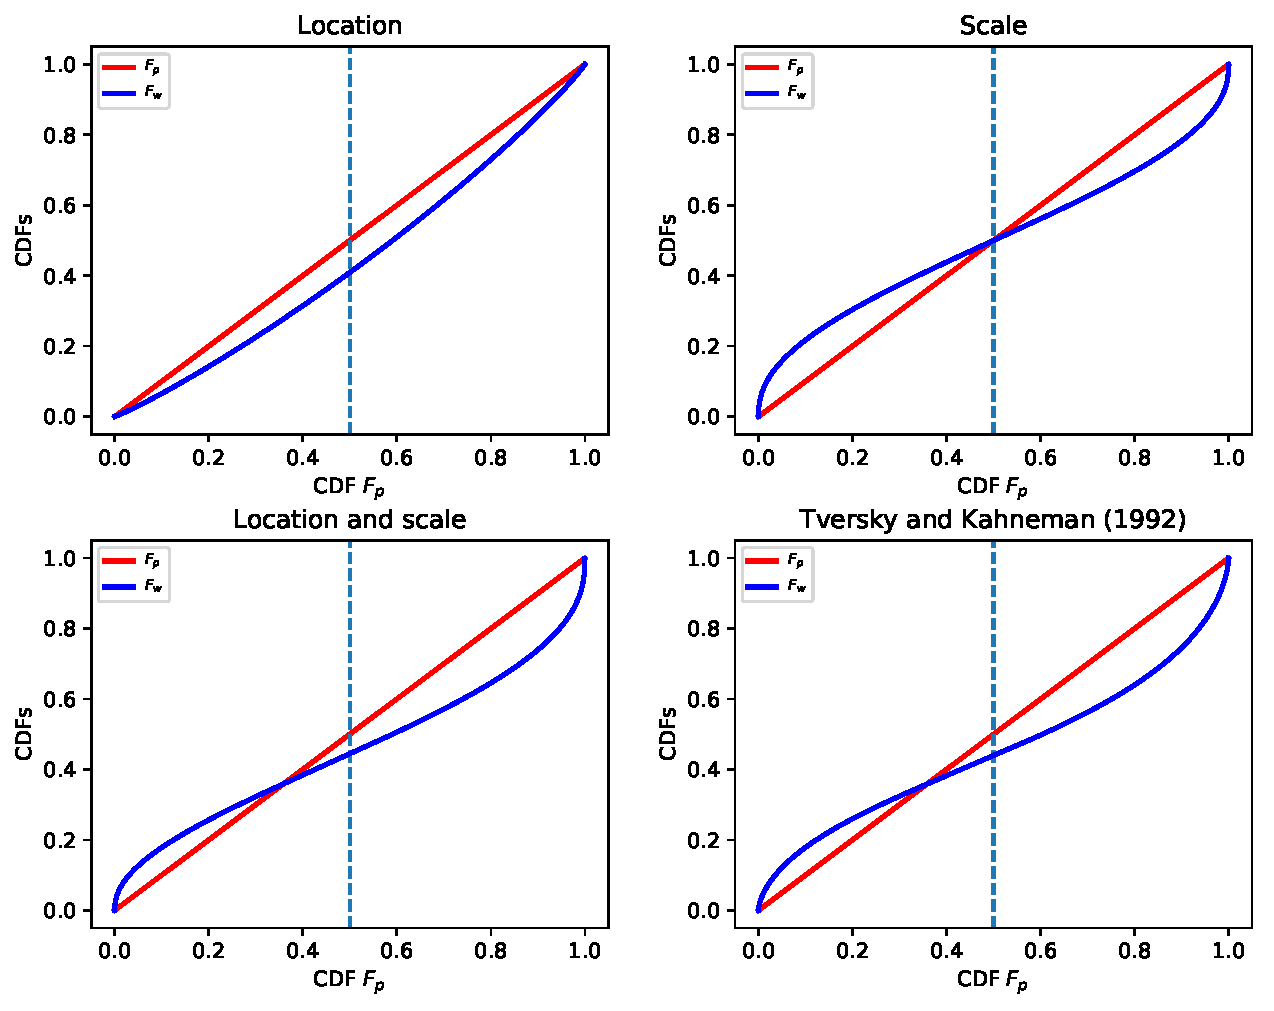
\includegraphics[width=1.0\textwidth]{./figs/Gauss_scale_location_both_KT.pdf}
 \caption{{\bf CDF maps, Gaussian distribution}.\\ 
 Top left: Difference in scale. DO assumes location 0, scale 1; DM assumes location 0, scale 1.64 (broader than DO).\\ 
 Top right: Difference in location. DO assumes location 0, scale 1; DM assumes location 0.18 (bigger than DO), scale 1.\\
 Bottom left: Differences in scale and location. DO assumes location 0, scale 1; DM assumes location 0.18 (bigger than DO), scale 1.64 (broader than DO).\\ 
 Bottom right: Fit to observations reported by \cite{TverskyKahneman1992}. This is \eref{correspondence} with $\gamma=0.65$.
Note the similarity to bottom left.}
 \flabel{CDF_weights}
 \end{figure}
 A difference in assumed scales and locations, for simple Gaussian distributions, is sufficient to reproduce the observations. This suggests a different nomenclature and a conceptual clarification. The inverse-S curve does not mean that ``probabilities are re-weighted'' -- it just means that experimenters and their subjects have different views about what might be an appropriate response to a situation. 

%% same figure using subfigure and reps. captions 
%\begin{figure}
%\begin{center}
%	\subcaptionbox{Gaussian distribution, difference in scale. DO assumes location 0, scale 1; DM assumes location 0, scale 2.7 (broader than DO).\flabel{subfig:GaussLocation}}
%	[.45\textwidth]{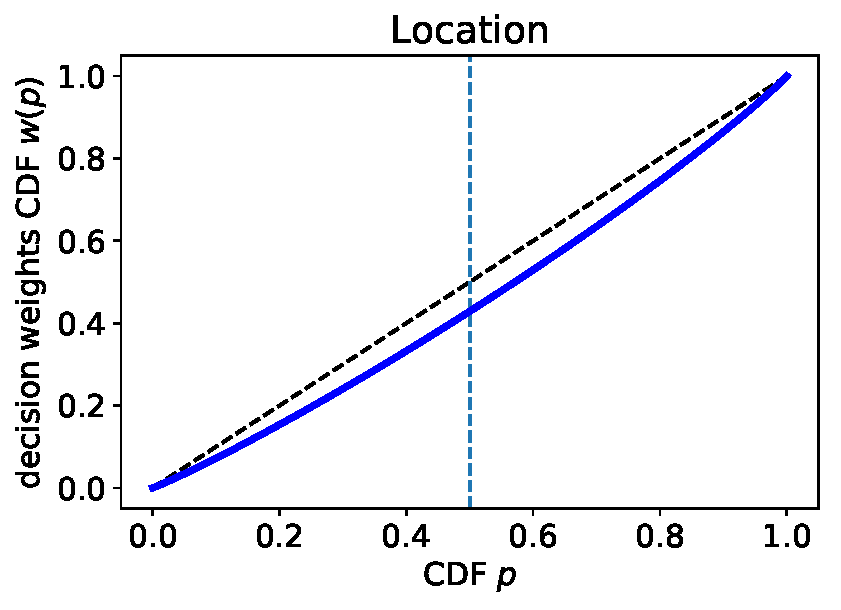
\includegraphics[width=.45\linewidth]{./figs/Gauss_location.pdf}}
%	\subcaptionbox{Gaussian distribution, difference in location. DO assumes location 0, scale 1; DM assumes location 0.18 (bigger than DO), scale 1.\flabel{subfig:GaussScale}}
%	[.45\textwidth]{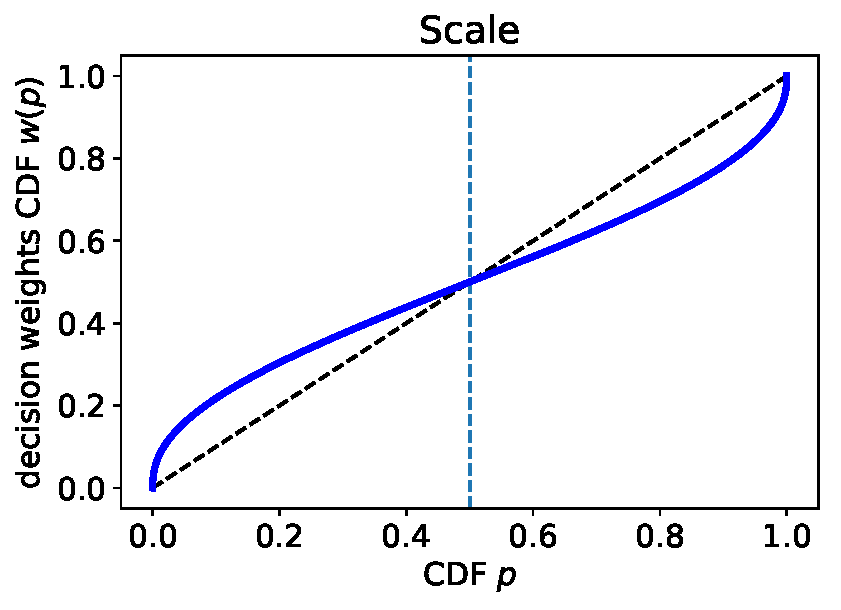
\includegraphics[width=.45\linewidth]{./figs/Gauss_scale.pdf}}
%	\\
%	\subcaptionbox{Gaussian distribution, differences in scale and location. DO assumes location 0, scale 1; DM assumes location 0.18 (bigger than DO), scale 2.7 (broader than DO).\flabel{subfig:GaussLocScale}}
%	[.45\textwidth]{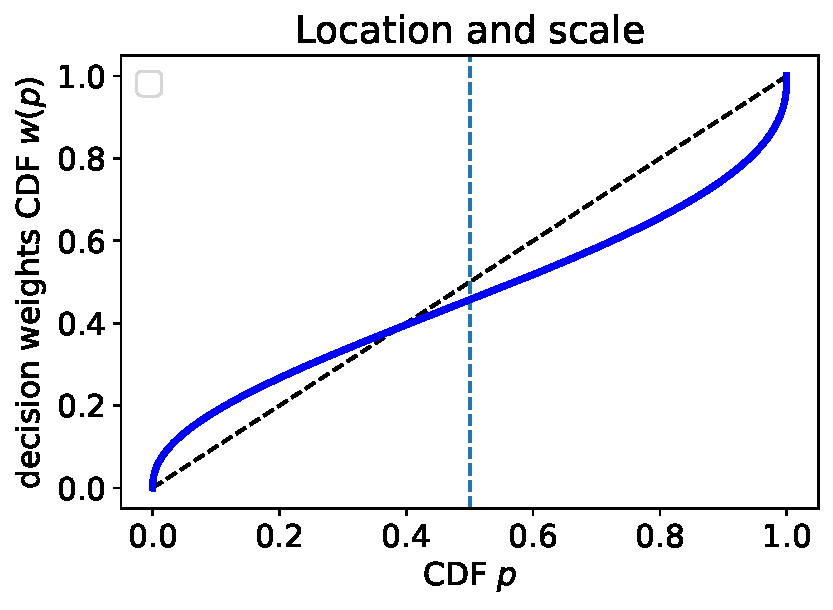
\includegraphics[width=.45\linewidth]{./figs/Gauss_location_and_scale.pdf}}
%%
%	\subcaptionbox{The observations by \cite{TverskyKahneman1992} are consistent with a DM assuming a scale and location in real-world decisions that differ from those assumed by the DO.\flabel{subfig:PW_TK}}
%	[.45\textwidth]{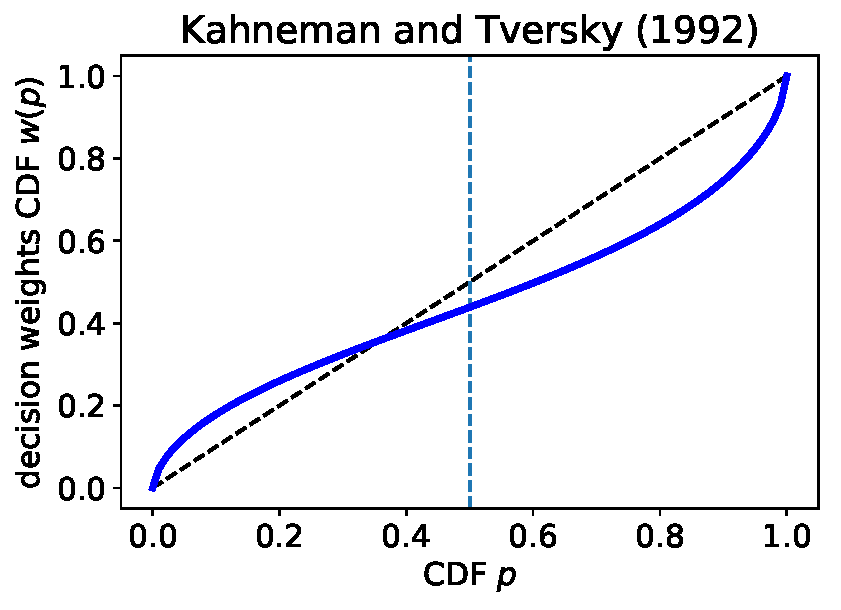
\includegraphics[width=.45\linewidth]{./figs/KT1992.pdf}}
%% 	\vspace{1em}
%\caption{{\bf Effects of differences in location and scale for the decision weight CDFs used by a DM vs. probability CDFs used by a DO.}\\
%\MK{Some more summarising text?}
%% Top left) Gaussian distribution, difference in scale. DO assumes location 0, scale 1; DM assumes location 0, scale 2.7 (broader than DO).\\ 
%% Top right) Gaussian distribution, difference in location. DO assumes location 0, scale 1; DM assumes location 0.18 (bigger than DO), scale 1.
%% Bottom left) Gaussian distribution, differences in scale and location. DO assumes location 0, scale 1; DM assumes location 0.18 (bigger than DO), scale 2.7 (broader than DO).\\ 
%% Bottom right) Fit to observations reported by \cite{TverskyKahneman1992}. This is \eref{correspondence} with $\gamma=0.65$.
%% The observations by \cite{TverskyKahneman1992} are consistent with a DM assuming a scale and location in real-world decisions that differ from those assumed by the DO.
%\flabel{CDF_weights}
%\MK{Double check parameter values with py source code}
%}
%\end{center}
%\end{figure}

\FloatBarrier
\subsection{Different shapes\seclabel{Different_shapes}}
Numerically, our procedure can be applied to arbitrary distributions: 
\begin{enumerate}
\item
construct a list of values for the CDF assumed by the DO, $F_p(x)$.
\item
construct a list of values for the CDF assumed by the DM, $F_w(x)$.
\item
plot $F_w(x)$ vs $F_p(x)$.
\end{enumerate}
Of course, the DM could even assume a distribution whose shape differs from that of the DO's distribution. 
%An infinity of combinations of assumed distributions can be explored. 
The inverse-S arises whenever a DM assumes a greater scale for a unimodal distribution. 
To illustrate the generality of the procedure, in \fref{fat_tailed_CDF} we carry it out for Student's (power-law tailed) $t$-distributions (which we refer to as $t$-distributions), where DO and DM use different shape parameters and different locations.\footnote{The PDF of the $t$-distribution is
%
\be
f\left(x\right) = \frac{\Gamma\left(\frac{\nu+1}{2}\right)} {\Gamma\left(\frac{\nu}{2}\right)\sqrt{\pi\nu}\sigma} \left(1+\frac{1}{\nu}\left(\frac{x-\mu}{\sigma}\right)^2 \right)^{-\frac{\nu+1}{2}}\,,
\ee
%
where $\nu$ is the shape parameter, $\sigma$ is the scale parameter, and $\mu$ is the location parameter. The corresponding CDF is
%
\be
F\left(x\right) = 
\begin{cases}
1 - \frac{1}{2} I_{\frac{\nu}{\left(\frac{x-\mu}{\sigma}\right)^2 + \nu}}\left(\frac{\nu}{2},\frac{1}{2}\right) &\text{ if } x-\mu \geq 0\,;\\
\frac{1}{2} I_{\frac{\nu}{\left(\frac{x-\mu}{\sigma}\right)^2 + \nu}}\left(\frac{\nu}{2},\frac{1}{2}\right) &\text{ if } x-\mu < 0\,,
\end{cases}
\ee
%
where $I_x\left(a,b\right)$ is the incomplete beta function.

In the limit $\nu \rightarrow \infty$, the $t$-distribution converges to a Gaussian with location $\mu$ and scale $\sigma$. We assume by default that $\sigma = 1$, so the $t$-distribution is effectively characterised by two parameters -- shape ($\nu$) and location ($\mu$).
}
The result is qualitatively similar to the bottom right panel of \fref{TwoCDFs}, corresponding to \eref{correspondence}. 



\begin{figure}[htb]
\centering
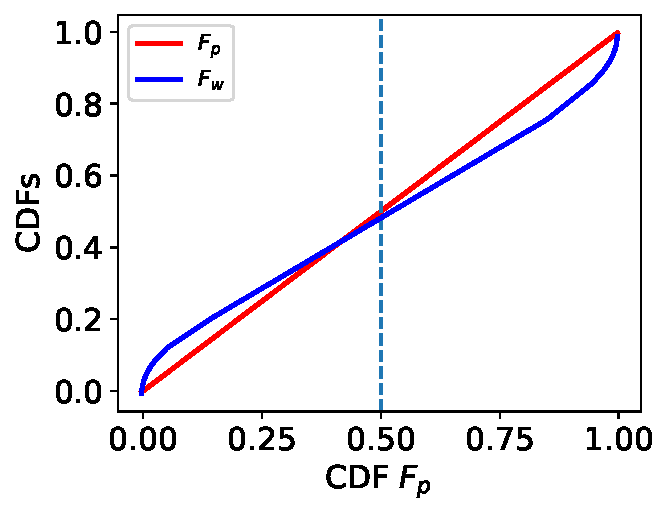
\includegraphics[width=0.5\textwidth]{./figs/Student-t.pdf}
\caption{Probability weighting for $t$-distributions, where the DM uses a different shape parameter (1) and a different location parameter (0) from those of the DO (2 and 0.2, respectively).}
\flabel{fat_tailed_CDF}
\end{figure}

%We denote these by $F_p=\int_{-\infty}^x p(s) ds$ (for the DO) and by $F_w=\int_{-\infty}^x w(s) ds$ (for the DM). 
%We will use the terms scale and location, rather than mean and standard deviation, to emphasise the generality of our arguments: 

%To clarify this nomenclature: starting with the standard form of a distribution $P(x)$ (of scale 1 and location 0), for example $P_{\text{standard}}(x)\sim \ND(0,1)$, the corresponding distributions of scale $\sigma$ and location $\mu$ are obtained by transforming $x$. With $y=\frac{x-\mu}{\sigma}$, we have $P_{\text{standard}}(y)=\ND(\mu, \sigma^2)$.

\FloatBarrier
\section{Reasons for different models\seclabel{Reasons_for}}
``Probability weighting'' is a term that suggests a detrimental cognitive bias, and the empirical findings are often interpreted that way. We caution against this interpretation. At least we should keep in mind that it is unclear who suffers from the bias: experimenter or test subject? 

Whatever the answer, two observations are robust and interesting: first, disagreement is common; and, second, the disagreement tends to go in the same direction: DMs tend to assume a greater range of plausible outcomes than DOs. 

%The first observation raises the question why disagreement about probabilities used in a model is common; the second, there must be a reason for such disagreement to be consistent: there must be a relevant systematic difference between the DO and the DM. 

An explanation for the first observation is that probability is a slippery concept, and the word is used to mean different things. 
%Even once one has settled on a definition, numerical values for probabilities are still difficult to estimate from real-world observations (see \secref{tricky}).
The second observation may be explained as follows. A DO often has control over, and essentially perfect knowledge of, the decision problem he poses. A DM does not have such knowledge, and this ignorance will often translate into additional assumed uncertainty. For example, the DO may know the true probabilities of some gamble in an experiment; the DM may in addition have doubts about the DO's sincerity, or whether he (the DM himself) fully understands the rules of the game. We will return to this in \secref{condition2}.

\subsection{Some meanings of ``probability'' \seclabel{tricky}}

Many thousands of pages have been written about the meaning of probability. We will not attempt a summary of the philosophical debate and instead highlight a few relevant points.
%systematically different incentives from a real-world DM. The DO tends to have an incentive to estimate, or indeed state, probabilities as their most likely value or ``true'' value (if the DO can control the probabilities, \eg in an experiment); the DM simply strives to behave optimally under uncertainty, and that uncertainty often includes uncertainty about the probabilities or model parameters.

%The conundrum surrounding the observed phenomenon of the characteristic inverse-S-shaped probability weighting vanishes if probability is understood as individual ignorance, \ie somebody's uncertainty about an observable.

\paragraph{Frequency-in-an-ensemble interpretation of probability}
Consider the simple probabilistic statement: ``the probability of rain here tomorrow is 70\%.'' Tomorrow only happens once, so one might ask: in 70\% of what will it rain? The technical answer to this question is often: rain happens in 70\% of the members of an ensemble of computer simulations, run by a weather service, of what may happen tomorrow. So one interpretation of ``probability'' is ``relative frequency in a hypothetical ensemble of simulated possible futures.'' 

It is thus a statement about a model. How exactly it is linked to physical reality is not completely clear. 

%Sometimes ensembles are real, for instance, when we say the probability of having a car accident is 1\% per 10000 km driven -- that's a summary of statistics collected over a large ensemble of cars. In this case, it's a real ensemble that existed in the past, not an imagined one in the future. 

\paragraph{Frequency-over-time interpretation of probability}
In some situations, the statement ``70\% probability of rain here tomorrow'' refers to the relative frequency over time. Before the advent of computer models in weather forecasting, people used to compare recent measurements (of wind and pressure today, say) to measurements further in the past -- weeks, months, years earlier, that were similar and where one had reason to believe that what had happened 1 day later would be similar to what would happen tomorrow.

Rather than a statement about outcomes of an in-silico model, the statement may thus be a summary of real-world observations over a long time.

\paragraph{Degree-of-belief interpretation of probability}
No matter how ``probability'' relates to a frequentist physical statement (whether with respect to an ensemble of simultaneously possible futures or to a sequence of actual past futures), it also corresponds to a mental state of believing something with a degree of conviction: ``I'm 90\% sure I left my wallet in that taxi.''

For our purpose it suffices to say that there's no guarantee that a probabilistic statement will be interpreted by the receiver (the DM) as it was intended by whoever made the statement (the DO).

\subsection{Consistent differences between DO and DM \seclabel{condition2}}

\subsubsection*{Estimation errors for probabilities}
Let's assume that both the DO and the DM mean by ``probability'' the relative frequency of an event in an infinitely long time series of observations. Of course, real time series have finite length, so probabilities defined this way are model parameters and cannot actually be observed. But, from a real time series, we can estimate the best values to put into a model, by counting how often we see an event. 

As the probability of an event gets smaller, so does the number of times we see it in a finite time series. If we want to say something about the uncertainty in this number, we can measure it -- or imagine measuring it -- in several time series to see how much it varies. These variations across time series also get smaller for rarer events. However, the relative variations get larger, and so does the relative uncertainty in our estimate of probabilities for rare events. Take an extreme simplified example: asymptotically an event occurs in 0.1\% of observations and we have a time series of 100 observations. Almost all such series (around 99.5\% of them) will contain 0 or 1 events. Na\"{i}vely, then, we would estimate the probability as either 0 or 1\%. In other words, we would estimate the event as either impossible or occurring ten times more frequently than it really would in a long series. However, if the event occurs 50\% of the time asymptotically, then a probability estimate from 100 observations would likely (in around 95\% of series) be in the range 40--60\%, a much smaller relative error.

A DM who must estimate probabilities from observations is well advised to account for this behaviour of uncertainties in his decision-making. Specifically, the DM should acknowledge that, due to his lack of information, {\it prima facie} rare events may be rather more common than his data suggest, while common events, being revealed more often, are more easily characterised. In such circumstances, caution may dictate that the DM assign to rare events higher probabilities than his estimates, commensurate with his uncertainty in them. This would look like probability weighting to a DO and, indeed, would constitute a mechanistic reason for it.

Let's make a simple scaling argument and then check it with a simulation. For an asymptotic probability density $p(x)$, the number of events $n(x)$ we see in the small interval $[x, x+ \delta x]$ in a time series of $T$ observations is proportional to $p(x)$, to $\delta x$, and to $T$. So we have $n(x) \sim p(x) \delta x T$, where we mean by $\sim$ ``scales like.'' We also know that such counts, such as in the simple Poissonian case, are random variables whose uncertainties scale like $\sqrt{n(x)}$.

If we knew the asymptotic probability density $p(x)$, we could make an estimate of the count as
\be
n(x) \approx p(x) \delta x T \pm \sqrt{p(x) \delta x T}.
\elabel{count_est}
\ee
We would write $\hat{n}(x) \equiv p(x) \delta x T$ as the estimate of $n(x)$ and $\err(\hat{n}) \equiv \sqrt{p(x) \delta x T}$ as its uncertainty. Of course, this situation seldom applies, because usually we do not know $p(x)$.

Conversely, and more realistically, if we observe a count $n(x)$, then we can use the scaling $ p(x) \sim n(x)/T\delta x$ to make an estimate of the asymptotic probability density as
\be
p(x) \approx \frac{n(x)}{T\delta x} \pm \frac{\sqrt{n(x)}}{T \delta x}.
\elabel{prob_est}
\ee
We write $\hat{p}(x) \equiv n(x)/T\delta x$ as the estimate of $p(x)$, and
\be
\err(\hat{p}) \equiv \frac{\sqrt{n(x)}}{T \delta x} = \sqrt{\frac{\hat{p}(x)}{T \delta x}}
\ee
as its uncertainty, which we have expressed in terms of the estimate itself.

The standard error, $ \sqrt{\hat{p}(x)/T \delta x}$, in an estimated probability density shrinks as the probability decreases. However, the relative error in the estimate is $1/\sqrt{\hat{p}(x)T\delta x}$, which grows as the event becomes rarer. This is consistent with our claim, that low probabilities come with larger relative errors, and constitutes the key message of this section. Errors in probability estimates behave differently for low probabilities than for high probabilities: absolute errors are smaller for lower probabilities, but relative errors are larger. 

Let's assume that the DM is aware of the uncertainties in his estimates and, furthermore, that he does not like surprises. To avoid surprises, he adds the standard error to his estimate of the probability density, $\hat{p}(x)$, in order to construct his decision weight density, $w(x)$. In effect, he constructs a reasonable worst case for each of his estimates. After normalising, this conservative strategy yields
\be
w(x)=\frac{\hat{p}(x)+\sqrt{\frac{\hat{p}(x)}{T \delta x}}}{\int_{-\infty}^{\infty}\left(\hat{p}(s)+\sqrt{\frac{\hat{p}(s)}{T \delta x}}\right)ds}\,.
\elabel{weight_density}
\ee

The cautionary correction term is parametrised by $T\delta x$, which scales like the number of observations in $[x, x+\delta x]$. As $T\delta x$ grows large, the correction vanishes and both $w(x)$ and $\hat{p}(x)$ become consistent with the asymptotic density, $p(x)$. With perfect information, a DM need not adjust decisions to account for uncertainty.

Does our analysis, culminating in \eref{weight_density}, reproduce the stylised facts of probability weighting, in particular the inverse-S curve? We check in two ways. First, analytically, by applying the DM's cautionary correction in \eref{weight_density} directly to reference probability density functions. Second, by simulating the DM compiling counts of outcomes drawn from reference distributions, from which he estimates probability densities and their uncertainties. In both cases, we treat the DO as using the reference distribution to make his predictions of the DM's behaviour.

\Fref{square_root_error} shows the resulting PDFs and CDF mappings generated by setting $\hat{p}(x)$ in \eref{weight_density} to be the probability density functions for a Gaussian distribution and a fat-tailed $t$-distribution. Inverse-S curves are found for both distributions and the effect is more pronounced for the fat-tailed distribution.
\begin{figure}[htb]
\centering
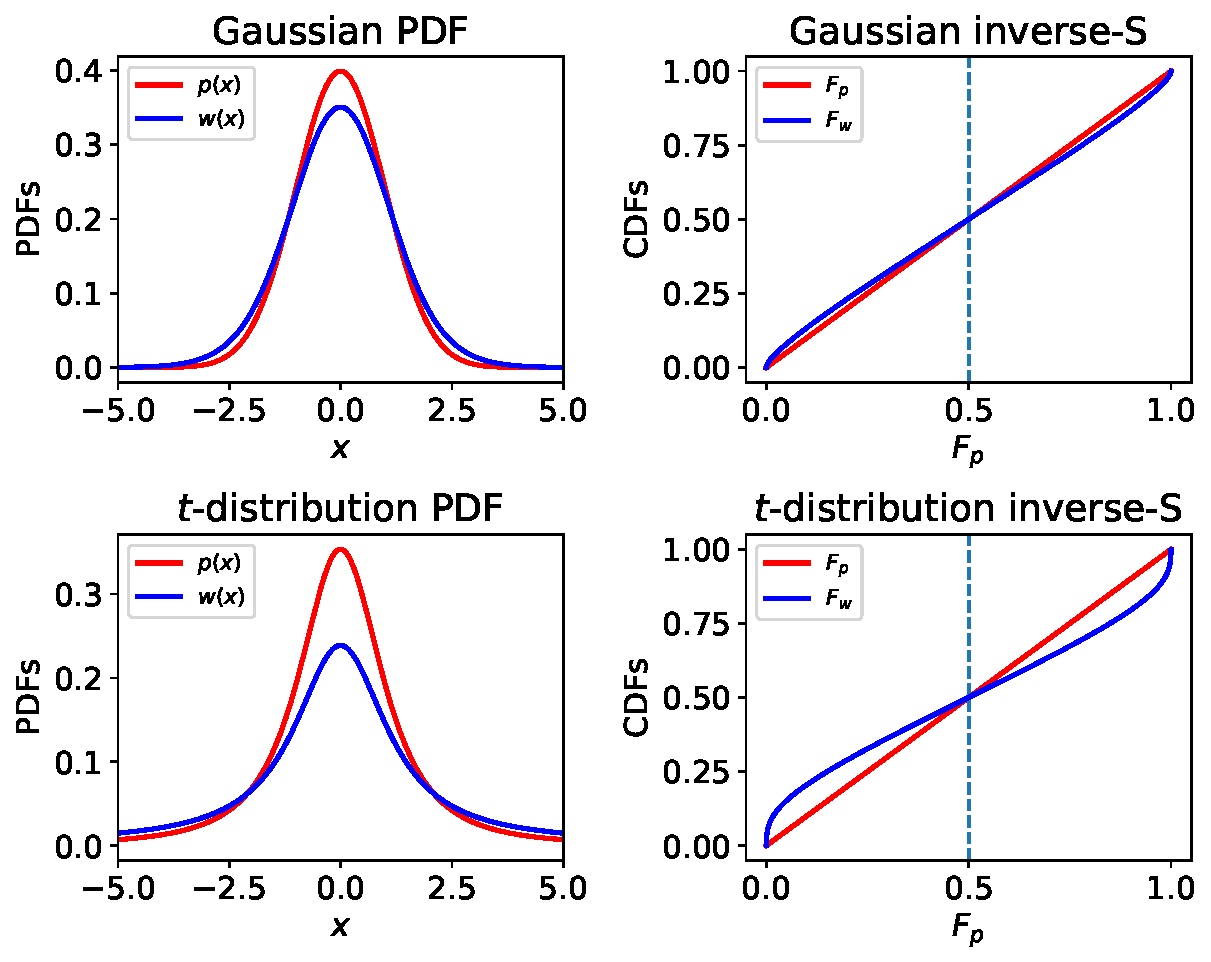
\includegraphics[width=1.0\textwidth]{./figs/square_root_error.pdf}
\caption{PDFs (left) and inverse-S curves (right) arising when the DO assumes a Gaussian (scale 1, location 0, top line) or a $t$-distribution (shape 2, location 0, bottom line), and the DM uses decision weights according to \eref{weight_density} with $T\delta x=10$. For the fat-tailed $t$-distribution (in the bottom line) the difference between $p(x)$ and $w(x)$ is more pronounced.}
\flabel{square_root_error}
\end{figure}

\Fref{dm_count_sim} shows the results of a computer simulation of a DM who observes a series of realisations of either Gaussian or $t$-distributed random variables, which he counts into bins. In the simulation, a probability density, $\hat{p}(x)$, is estimated for each bin as $n(x)/T\delta x$ and its uncertainty, $\err(\hat{p})$, is obtained numerically as standard deviation in each $\hat{p}(x)$ over 1000 parallel simulations. The DM's decision weights are then obtained according to \eref{weight_density}. Again, inverse-S curves are found for both distributions, corroborating our scaling arguments.
\begin{figure}[htb]
\centering
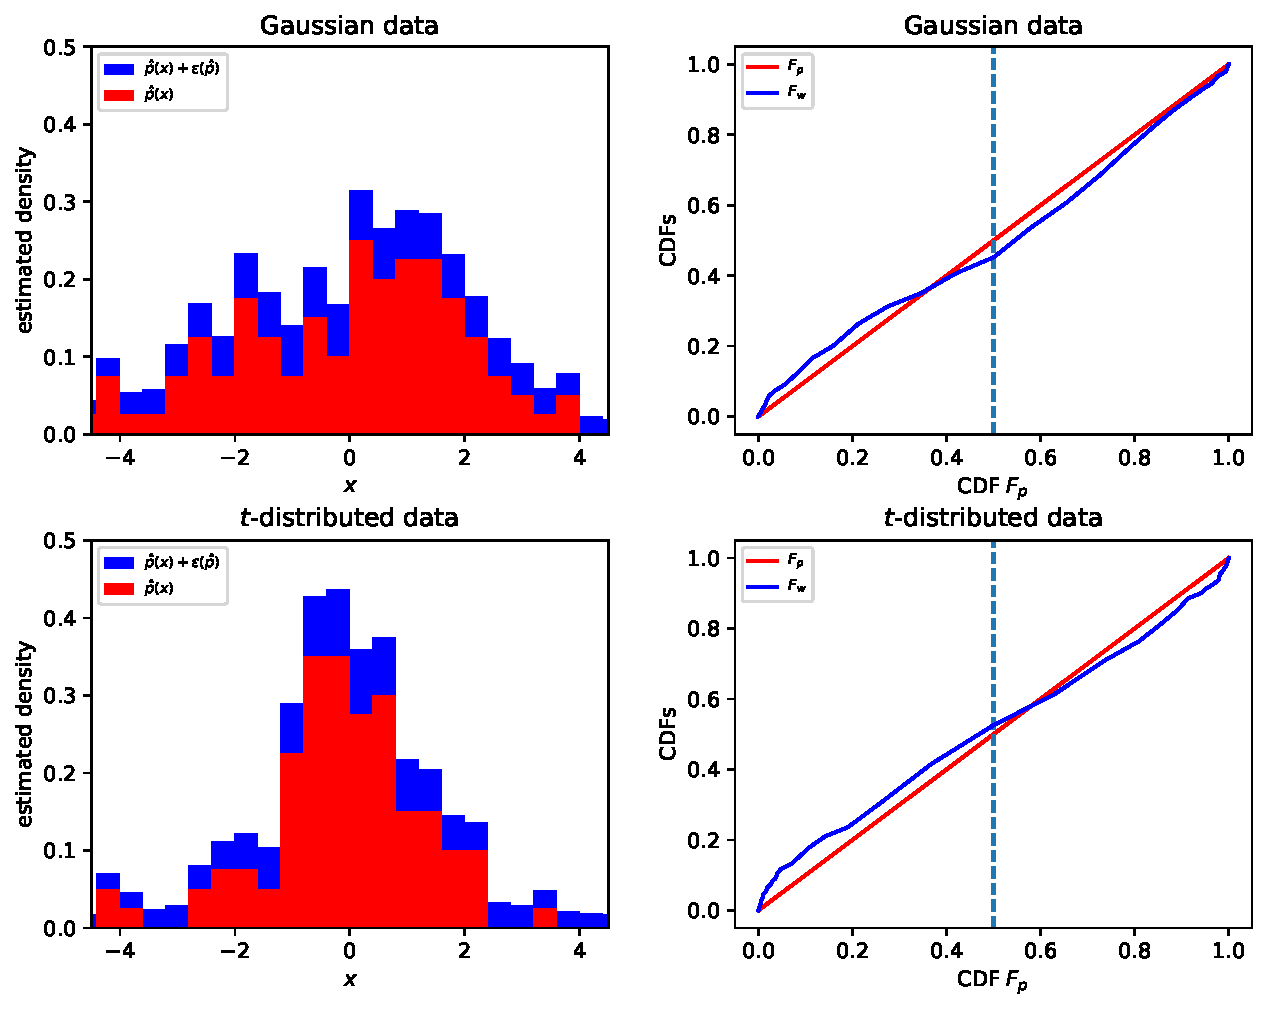
\includegraphics[width=1.0\textwidth]{./figs/dm_count_sim.pdf}
\caption{
Simulation of a DM estimating probability densities by counting events in a finite series of observations. Left: estimated probability densities for $T=100$ Gaussian (top; location 0, scale 2) and $t$-distributed (bottom; location 0, scale 1, shape 1.5) variates counted in bins of width $\delta x=0.4$. Red bars show the estimates, $\hat{p}(x)$, and blue bars show the estimates with one standard error added, $\hat{p}(x)+\err({\hat{p}})$. Right: inverse-S curves for a DO who assumes $p(x)$ follows a Gaussian (top) and $t$-distribution (bottom), while the DM uses decision weight density, $w(x)$, derived by normalising his conservative estimates (blue bars on left) according to \eref{weight_density}.
}
\flabel{dm_count_sim}
\end{figure}

\FloatBarrier
\subsubsection{Typical situations of DO and DM: ergodicity}
To recap: behavioural economics observes that DOs tend to assign lower weights to low-probability events than DMs.
While behavioural economics commonly assumes that the DM is wrong, we make no such judgement. In any decision problem, the aim of the decision must be taken into account, and that crucially depends on the situation of the individual. 

The two types of modellers (DO and DM) pursue different goals. Broadly, the DO tends to be a behavioural scientist without personal exposure to the success or failure of the DM (who tends to be a test subject or someone whose behaviour is being observed in the wild). The DM, of course, has such exposure. Throughout the history of economics, it has been a common mistake, by DOs, to assume that DMs optimise what happens to them on average in an ensemble. To the DM what happens to the ensemble is usually not a primary concern -- instead, the concern of the DM is what happens to him over time. Not distinguishing between these two perspectives is only permissible if they lead to identical predictions, meaning only if the relevant observables are ergodic \citep{Peters2019b}. 

It is now well known that this is usually not the case in the following sense: DMs are usually observed making choices that affect their wealth, and wealth is usually modelled as a stochastic process that is not ergodic. The ensemble average of wealth does not behave like the time average of wealth.

The most striking example is the universally important case of noisy multiplicative growth -- universal because it is the fundamental process that drives evolution: noise generates the diversity of phenotypes necessary for evolution and multiplicative growth (self-reproduction) is how successful phenotypes spread their traits in a population. This process operates on amoeba, as it does on forms of institutions, and on investment strategies.
%\citep{PetersAdamou2015a}

The simplest model of noisy multiplicative growth is geometric Brownian motion, $dx=x(\mu dt+\sigma dW)$. The average over the full statistical ensemble (often studied by the DO) of geometric Brownian motion grows as $\exp(\mu t)$. The individual trajectory of geometric Brownian motion, on the other hand, grows in the long run as $\exp[(\mu-\frac{\sigma^2}{2})t]$.

If the DO takes the ensemble perspective, he will deem the fluctuations irrelevant. But from the DM's time perspective, they reduce growth. While a DO interested in the ensemble may get away with disregarding low-probability events, for the DM's success hedging against rare events is of crucial importance (not only but ultimately also for survival).

The difference between how these two perspectives evaluate the effects of probabilistic events is qualitatively in line with the observed phenomena we set out to explain. The DM typically has large uncertainties, especially for low-probability events, and has an evolutionary incentive to err on the side of caution, \ie to behave as though low-probability (extreme) events had a higher probability than in the DO's model.


\section{Fitting the model to experimental results \seclabel{Fitting_the}}

Visually, looking at the figures and the level of noise in the data in \fref{TK1992}, one would conclude that Tversky and Kahneman's fitting exercise of the inverse-S curve by way of the physically unmotivated function $\tilde{F}^{TK}_w$, \eref{correspondence}, resembles the data no better than our mechanistically constrained model. This is particularly evident in the bottom two panels of \fref{CDF_weights}, which show that a Gaussian $w(x)$ whose scale and location differ from those of $p(x)$ reproduces the fitted functional shape of $\tilde{F}^{TK}_w$.

For completeness and scientific hygiene, in the present section we fit location and scale parameters in the Gaussian and $t$ models for $F_w$ to experimental data from \cite{TverskyKahneman1992} (depicted in circles in \fref{TK1992}) and from \cite{TverskyFox1995}. Specifically, in the Gaussian model we fit the location and scale parameters $\mu$ and $\sigma$ in the CDF
%
\be
F_w\left(x\right) = \Phi\left(\frac{\Phi^{-1}\left(F_p\left(x\right)\right) - \mu}{\sigma}\right)\,,
\ee
%
where $\Phi$ is the CDF of the standard normal distribution. In the $t$-model we fit the location parameter $\mu$ and the shape parameter $\nu$ in the CDF $F_w\left(x\right)$ of a $t$-distributed random variable (see \secref{Different_shapes}), assuming $p$ follows a standard normal distribution.

%For $\nu\to\infty$, the Student-t converges to the Gaussian, whereas $\nu=1$ is a very heavy-tailed Student-t (diverging variance). The Student-t arises in sampling when the variance is estimated from a sample of Gaussian random variates. So there's a reasonable motivation for comparing specifically Gaussian and Student-t.

In addition to \eref{correspondence} used by Tversky and Kahneman, we fit the function
%
\be
\tilde{F}^{L}_w\left(F_p; \delta,\gamma\right) =\frac{\delta F_p^{\gamma}}{\delta F_p^{\gamma} + \left(1-F_p\right)^{\gamma}}\,,
\elabel{LattimoreFunction}
\ee
%
suggested by \cite{LattimoreBakerWitte1992} to parametrically describe probability weighting (also used by \cite{tversky1995risk} and \cite{Prelec1998}). The reason for fitting \eref{LattimoreFunction} is to ensure a fair comparison: the Gaussian and $t$ models are characterised by two parameters, whereas \eref{correspondence} only has one free parameter. \Eref{LattimoreFunction} has two parameters.

\Fref{TK_TF_fit} presents the fit results. We obtain very good fits to data for both Gaussian and $t$-distributions, as well as for \eref{correspondence} and \eref{LattimoreFunction}, in the two experiments. It is practically impossible to distinguish between the fitted functions within standard errors. We conclude that our model fits the data well, and unlike \eref{correspondence} or \eref{LattimoreFunction}, the fitted functions are directly derived from a physically plausible mechanism, and are not simply phenomenological.

\begin{figure}[htb]
\centering
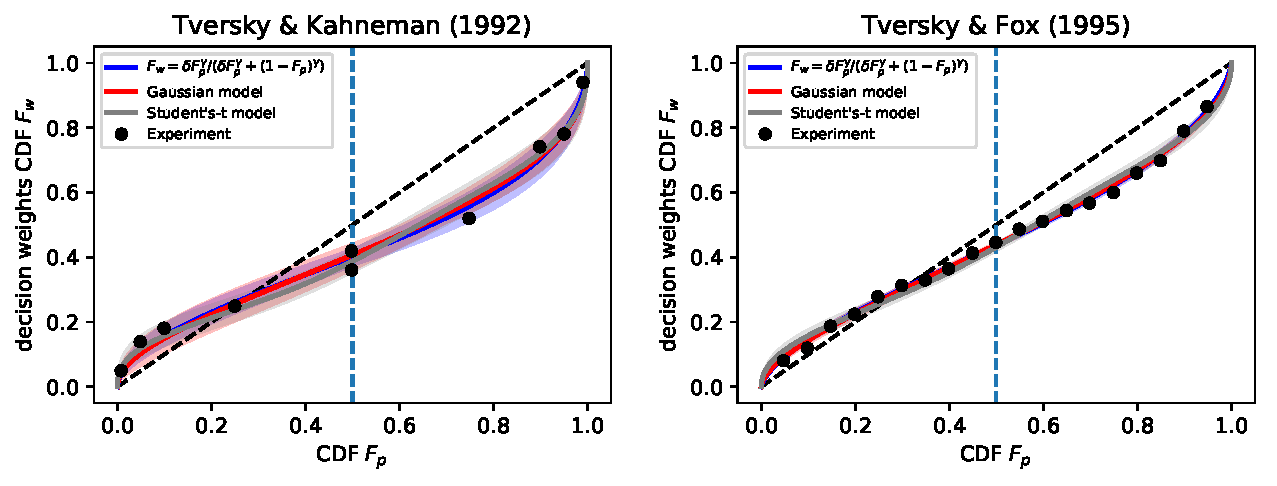
\includegraphics[width=1.0\textwidth]{./figs/TK_TF_curvefit.pdf}
\caption{Model fitting to experimental data from \cite{TverskyKahneman1992} (left) and \cite{TverskyFox1995} (right).
Left: \cite{LattimoreBakerWitte1992} \eref{LattimoreFunction}: $\delta=0.67\,\left(SE = 0.04\right)$, $\gamma=0.58\,\left(\pm0.03\right)$; Gaussian model: $\mu=0.38\,\left(\pm0.06\right)$, $\sigma=1.60\,\left(\pm0.10\right)$; $t$-model: $\nu=1.27\,\left(\pm0.28\right)$, $\mu=0.40\,\left(\pm0.07\right)$; \cite{TverskyKahneman1992} \eref{correspondence}: $\gamma=0.60\,\left(\pm0.02\right)$. Right: \cite{LattimoreBakerWitte1992}: $\delta=0.77\,\left(\pm0.01\right)$, $\gamma=0.69\,\left(\pm0.01\right)$; Gaussian model: $\mu=0.22\,\left(\pm0.01\right)$, $\sigma=1.41\,\left(\pm0.03\right)$; $t$-model: $\nu=1.41\,\left(\pm0.21\right)$, $\mu=0.22\,\left(\pm0.03\right)$; \cite{TverskyKahneman1992}: $\gamma=0.68\,\left(\pm0.01\right)$. Shaded areas indicate two standard errors in the fitted parameter values. The fit was done by implementing the Levenberg-Marquardt algorithm \cite{Levenberg1944} for non-linear least squares curve fitting.
%The fit was done by implementing the method of least squares with the Nelder-Mead algorithm \cite{NelderMead1965}, and the standard errors were obtained by bootstrapping.
}
\flabel{TK_TF_fit}
\end{figure}

\FloatBarrier

\newpage
\section{Discussion}
% \OP{We could move some discussion bits here -- like the incredible Sunstein story.}
% \MK{Discuss the general action of change of measure in relation to Girsanov and risk-neutral prob measure $\mathbb{Q}$ in Math Finance?}
% \OP{Let's keep this paper focused on one point only.}
On 28 February 2020, \citet{Sunstein2020}, a behavioural economist, legal scholar, and former United States Administrator of the Office of Information and Regulatory Affairs, diagnosed that people's concern about a potential coronavirus outbreak in the US was attributable to an extreme case of probability weighting -- they neglected the fact, supposedly, that such an event had a low probability. When the piece was published, many commented that it seemed quite reasonable to them to take precautions, and Sunstein himself may have underestimated the severity of what lay ahead. One month later the US became the epicentre of the global coronavirus pandemic.

The episode illustrates that an inverted S-curve is a neutral indicator of a difference in opinion. It says nothing about who is right and who is wrong.

The term ``probability weighting'' suggests an obscure mental process, where a DM carries out operations on probabilities. It seems more natural to us to consider a DM modelling events he is unsure about. From this latter point of view, it is easy to think of reasons for a DM's model to differ from a DO's. Specifically DMs will often include additional uncertainty, leading to the frequently observed inverse-S shape.

% It suggests that DMs perceive the probability of an event, and combines regularities in experimental behaviour of human subjects, \ie the overestimation of rare events and consequently the underestimation of common events, which together generate the known inverse-S shape. As such probability weighting is a building block of decision models in behavioural economics and part of the fourfold pattern of risk attitudes.
%In this article we contribute to a mechanistic understanding of this empirical phenomenon.

%First, there are good reasons for the DM and the DO to use of different models or model parameters (see \secref{ModelDiff}) in reasoning about the same uncertain outcomes. It is no longer a question about who is right or wrong, rational or irrational.
 
%Second, accepting the difference in models, the valid question asks for the explanation of qualitative properties of the difference in models.
%
The model of estimating probabilities from real time series, which we discuss in \secref{Reasons_for} has qualitative features that display a degree of universality. Relative errors in the DM's probability estimates are always greater for rarer events. A dislike of the unexpected, which explains the systematic overestimation of low probabilities, is similarly common. ``Probability weighting'' is purely descriptive and comes with the ill-conceived connotation of DMs suffering from a cognitive error. The phenomenon is better thought of as DMs making wise decisions given the information available to them, which is constrained because they must collect such information as time passes.

% \paragraph{Related literature}
% 
% \cite{WuGonzalez1996,Prelec1998}: derive PW from preference axioms, goal is to generate concavity and then convexity
% 
% \cite{Stott2006}: test several functional forms, corroborate \cite{Prelec1998} and \eref{correspondence} and \eref{LattimoreFunction}, respectively. None of the tested functional forms corresponds to the function we derived mechanistically in \eref{w_of_p}. 
% 
% \cite{Wakker2010}: the whole book contains only parameter calibrations of \eref{correspondence} but provides no mechanistic explanation.
% 
% \cite{AbdellaouiETAL2011}: maybe closest to what we do in terms of their Fig. 2., however they distinguish between source functions for ambigious probabilities and known probabilities. They interpret the shifts and shape of the inverse-S curve using two additional idiosyncratic psychological parameters encoding optimism(pessimism) and likelihood (in)sensitivity. 

% Whereas we provide a mechanistic explanation, psychological explanations prevail in the behavioural economics and finance literature, see \cite{WuGonzalez1996,Prelec1998,GonzalezWu1999,Stott2006,DeGiorgi2006,Wakker2010,AbdellaouiETAL2011} and references especially in the latter. It remains doubtful how a psychological explanation shall compensate for a missing and/or not yet understood mechanism, generating a particular phenomenon like probability weighting.
% \OP{I think I see the point, but I don't know what a ``psychological explanation'' is; it may also be unclear what we mean by ``mechanistic.''}


% \paragraph{Results set in perspective}
% The consensus view hold in behavioural economics is that a descriptive decision model needs to feature 
% the so-called fourfold pattern of risk attitudes:
% \begin{enumerate}
% 	\item gain/loss asymmetry (kink at the reference point),
% 	\item nonlinearity in probability weighting (inverse-S curve),
% 	\item risk aversion for most gains \& low probability losses (concavity) and
% 	\item risk seeking for most losses \& low probability gains (convexity).
% \end{enumerate}
% All of these empirical patterns are usually (mis)interpreted as a deviation from \textit{the one and only} ``correct'' model and perceived as detrimental cognitive biases \citep{Lopes1991,Gigerenzer2018}. 
% % 
% Thus the mode of explanation in behavioural economics is to utilise psychological biases and cognitive processes in the brain which cause certain empirical regularities, \eg inverse-S curve labelled as probability weighting.
% %
% From a normative point of view there remains the desideratum to provide a mechanistic explanation for each of these patterns. Our contribution is that we provide a mechanistic explanation for probability weighting and show that it may even be adaptive in the likely case of cautiously using a model with more uncertainty relative to another model.



%\MK{End on a positive note}
%\MK{It has almost become custom to end with a Kacelnik quote}

% BibTeX users please use one of
\bibliographystyle{apalike}
\bibliography{../LML_bibliography/bibliography} % name your BibTeX data base
\end{document}